% !TEX encoding = UTF-8 Unicode

\documentclass[twocolumn,10pt,a4j]{ltjsarticle}
\usepackage{kougai}
\usepackage{enumitem}

\title{待ち行列問題シミュレータの開発}
\author{1932008 伊豆原嵩章 指導教員 須田 宇宙 准教授}
\date{}

\begin{document}

\maketitle

\section{はじめに}
病院の受付,店舗や交通渋滞など我々の生活の至る所に待ち行列が存在する.
行列による問題は多岐にわたり生産コストや回転率など,店舗の経営などに大きく関わってくる.
それら問題のアプローチ法としてモンテカルロ法を用いた待ち行列問題が存在し,シミュレーションを行うことでリソースを適正に算出し配備することができる.

また数値計算の授業において実際に教科書や黒板からの情報だけでは直感的に理解することが困難である.
そしてモンテカルロ法の一種である「待ち行列問題」があるが,数式にパラメータを代入して答えを算出する問題と違い,教科書のような静的な教材のみでは理解しずらい.
実際に解こうとしても高い精度の解を出すために数万回程度の試行が必要となり手計算での確認は困難である.

そして先行研究として視覚的・直感的に理解できることを目的とした待ち行列問題シミュレータが存在するが,開発環境が古く現在は使用できないこと,アニメーションが画像を切り替えていくことによる擬似的なアニメーションであり,なめらかなアニメーションではなかった.\cite{past}

そこでアニメーションをより現実的な動きに寄せブラウザ上への移植及び改良することでより利用者の理解度の向上が見込めると考えた.
本研究では待ち行列についてアニメーションを用いたシミュレータ教材をブラウザ上で開発することを目的とする.

\section{待ち行列の問題について}
待ち行列の問題とは,n 箇所の窓口が開いていてサービスに $\delta$時間かかる時の窓口で客がサービスで受けられるまでの平均待ち時間 t を計算することである.
このとき(N+1)番目の客が入ってくる時刻$t_{N+1}$は下記の式で表すことができる.\cite{text}\\
\vspace{-11mm}
\begin{eqnarray}
t_{N+1}=t_N+\tau\\
t_0=0\\ 
\tau=-\frac{1}{\alpha}\ln\gamma
\end{eqnarray}
同様に,個々の客のサービス時間は以下の式で表せれる.\\ 
\vspace{-5mm}
\begin{equation}
\delta=\delta_0+\sigma\nu
\end{equation}
\vspace{-1mm}
(\tau:次の客が入ってくる時間間隔の期待値,\alpha:客の流れの密度,\gamma:区間(0,1)の一様乱数,\delta:客一人が受けるサービスの時間,$\delta_0$:サービスに必要な平均時間,\sigma:標準偏差,$\nu=\gamma_1+\gamma_2+・・・+\gamma_{12}-6$)
実際に待ち行列問題を解くためには以下の4つのパラメータを定め,乱数を発生させて計算していく.\\
 (i)客の流れ密度\alpha\\
 (ii)窓口の数n\\
 (iii)サービスに必要な平均時間$\delta_0$\\
 (iv)サービスに必要な時間の標準偏差\sigma\\

N番目の客はどこかの窓口が空いていればその場所でサービスを受けられるが,全てが使用中だといずれかの窓口が空くまで待たされる.
この待ち時間を集積し全客数で割れば一人当たりの平均待ち時間が計算される.
しかし実際には営業時間や曜日等によって客の入ってる分布が異なるため,乱数などの偶発的な確率変数を用いて試行錯誤的に問題を解いていく数値計算法である.


\section{シミュレータ教材について}
図\ref{fig:教科書}は開発したシミュレータ教材のレイアウトである.
過去の卒業研究では問題点であるどのような状況遷移を経てその結果になったか理解することが難しいということから,ユーザーによる入力を行い実行することでアニメーション・グラフの遷移が始まり,状況の遷移を学ぶことできた.
しかし,開発環境が古く現在は使用できないこと,アニメーションが画像を切り替えていくことによる擬似的なアニメーションであり,なめらかなアニメーションではなかった.

そこでアニメーションをより現実的な動きに寄せブラウザ上への移植及び改良することでより利用者の理解度の向上が見込めると考えた.
パラメータの変更はユーザーの任意となっており,パラメータの変化によって待ち行列にどう変化が起こすか学ぶことができる.

①では各パラメータの設定をユーザーによって変更できる.
窓口の平均処理時間は1〜10,処理時間と流れ密度は0〜1の間で変更できるようにした.
②では平均待ち時間をグラフを表示する.
平均待ち時間の遷移を可視化し,安定状態が理解しやしくなると考えた.
③ではユーザーが設定したパラメータに応じて,アニメーションが実行される.
アニメーションにより現象をより直感的に理解できると考えた.

\begin{figure}[h]
\begin{center}
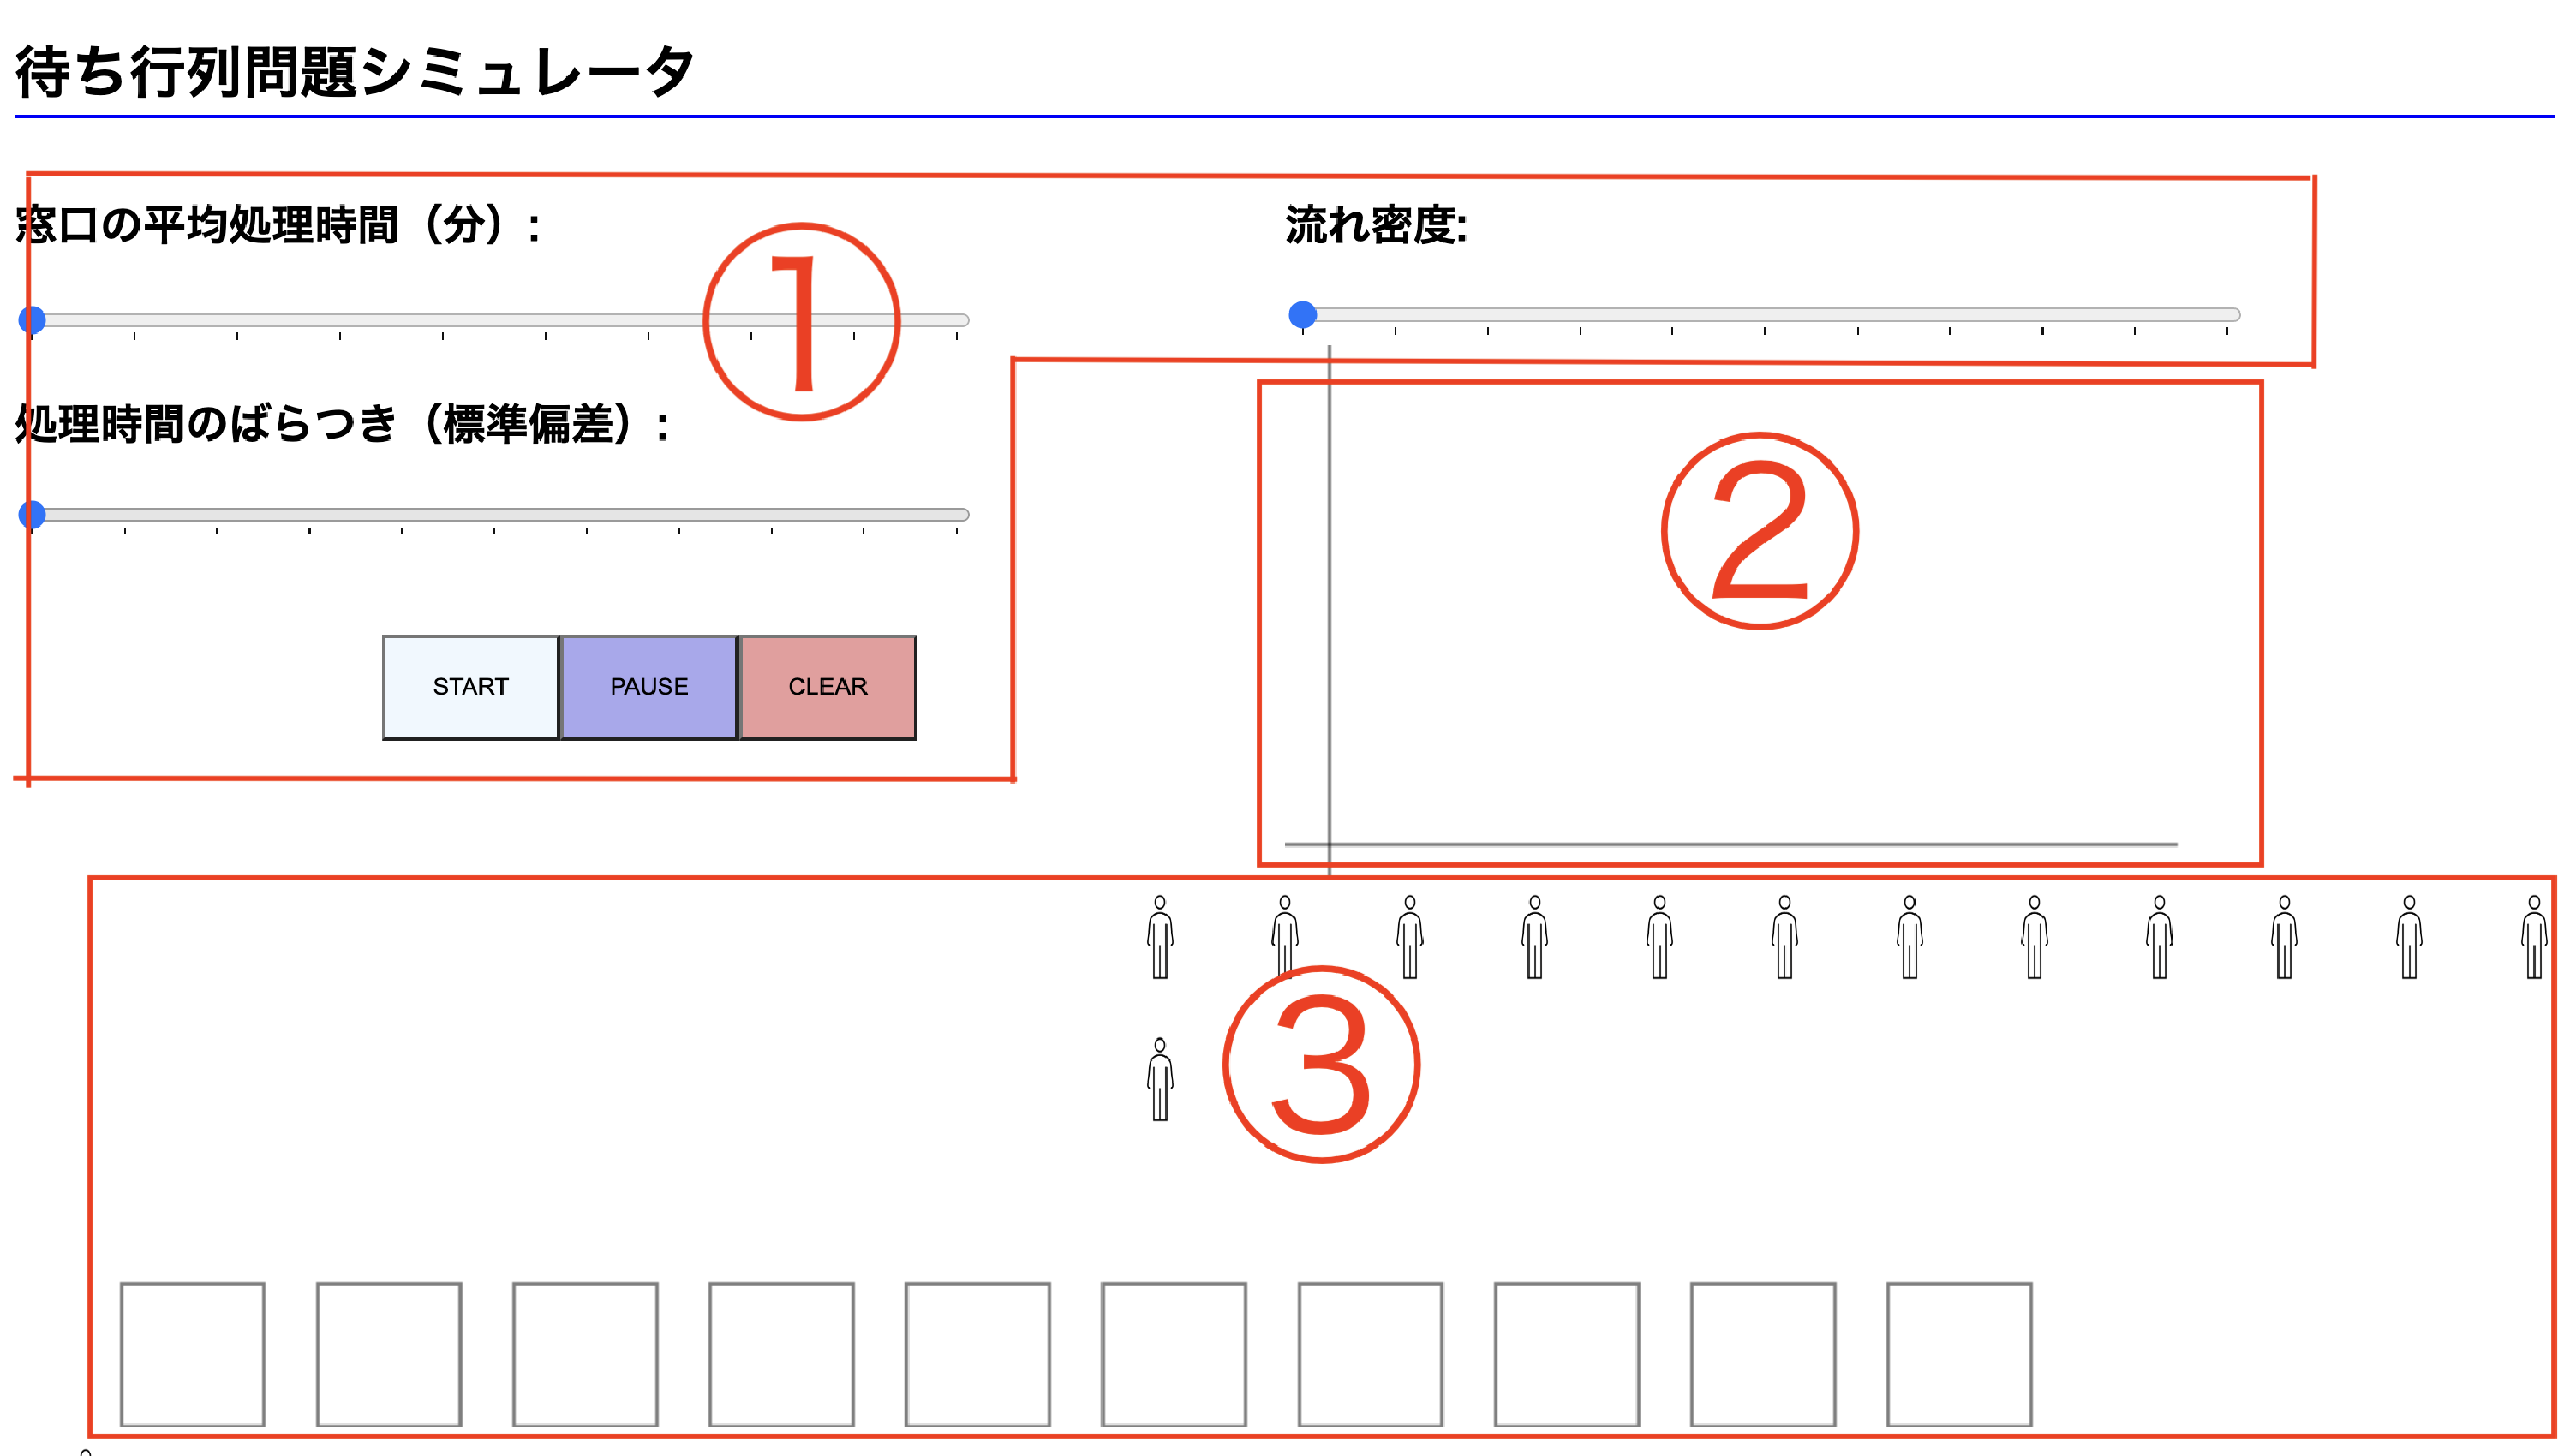
\includegraphics[clip,width=85mm,height=50mm]{figures/layout_ex.pdf}
\end{center}
\caption{シミュレータ教材スクリーンショット}
\label{fig:教科書}
\end{figure}

\section{おわりに}
本研究では,待ち行列についてアニメーションを用いたシミュレータ教材の開発を行った.しかし,技術的な問題で未対応の動作が多く,教材としては不十分なものとなってしまった.

\begin{thebibliography}{99}
\bibitem{past}平成16年度 卒業論文 薄井英彦・梅山卓也 モンテカルロ法による待ち行列問題のマルチメディア教材
 \bibitem{text}第2版 数値計算法 三井田 惇郎・須田 宇宙 共著
\end{thebibliography}
\end{document}
